\chapter{Sets}
\signature

\section{Definition}

\begin{definition}[Set]
A \emph{set} is an unordered collection of distinct objects, called its
\emph{elements} (or members). We write $a \in A$ when $a$ is an element of
$A$, and $a \notin A$ otherwise.
\end{definition}

Sets can be described by \emph{extension} (listing):
$A = \{1, 2, 3, 5, 8\}$, or by \emph{comprehension} (a defining property):
$A = \{x \in \N \mid x \text{ is a Fibonacci number} \le 8\}$. Order and
repetition are irrelevant: $\{1,2,2,3\} = \{3,2,1\}$.

\begin{definition}[Equality]
Two sets are equal when they have exactly the same elements:
$A = B \iff \forall x\,(x \in A \leftrightarrow x \in B)$
(the \emph{extensionality} principle).
\end{definition}

\section{Cardinality}

\begin{definition}
If $A$ contains exactly $n$ distinct elements ($n \in \N$), $A$ is
\emph{finite} and its \emph{cardinality} is $|A| = n$. Otherwise $A$ is
\emph{infinite}.
\end{definition}

\begin{example}
$|\{a, b, c\}| = 3$; $|\varnothing| = 0$; $|\{\varnothing\}| = 1$ (a set
containing one element, namely the empty set); $\Z$ is infinite.
\end{example}

\section{Important sets}

\[
\N = \{0, 1, 2, \ldots\},\quad
\Z = \{\ldots,-1,0,1,\ldots\},\quad
\Q = \Bigl\{\tfrac{p}{q} \;\Bigm|\; p,q \in \Z,\ q \neq 0\Bigr\},\quad
\R,\quad \C .
\]
We write $\Z^{+}$ for the positive integers and $[a,b]$, $(a,b)$ for real
intervals. The chain $\N \subset \Z \subset \Q \subset \R \subset \C$ will be
used constantly.

\subsection{Countable and uncountable}

\begin{definition}
A set is \emph{countable} when it is finite or when its elements can be listed
in an infinite sequence indexed by $\N$ (equivalently, when it has the same
cardinality as $\N$, written $\aleph_0$). Otherwise it is \emph{uncountable}.
\end{definition}

$\Z$ is countable (list $0, 1, -1, 2, -2, \ldots$) and so is $\Q$; Cantor's
diagonal argument shows $\R$ is uncountable --- there are strictly more reals
than integers. Chapter~8 returns to cardinality via bijections.

\section{Venn diagrams}

A \emph{Venn diagram} represents sets as regions (typically discs) inside a
rectangle standing for the universal set $U$.

\begin{center}
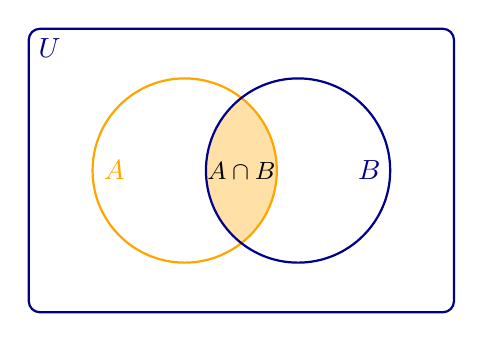
\begin{tikzpicture}[scale=0.9]
\draw[rounded corners,thick,color=DarkBlue] (-3,-2) rectangle (3,2);
\node[anchor=north west] at (-3,2) {\color{DarkBlue}$U$};
\begin{scope}
\clip (-0.8,0) circle (1.3);
\fill[Orange!35] (0.8,0) circle (1.3);
\end{scope}
\draw[thick,color=Orange] (-0.8,0) circle (1.3) node[left=18pt] {$A$};
\draw[thick,color=DarkBlue] (0.8,0) circle (1.3) node[right=18pt] {$B$};
\node at (0,0) {\small$A \cap B$};
\end{tikzpicture}
\end{center}

Venn diagrams guide intuition for the operations of Chapter~7, but a picture
is not a proof: identities must be established by the element method or by
membership tables.

\section{Subsets}

\begin{definition}
$A$ is a \emph{subset} of $B$, written $A \subseteq B$, when every element of
$A$ belongs to $B$: $\forall x\,(x \in A \to x \in B)$. If moreover
$A \neq B$, $A$ is a \emph{proper} subset, written $A \subset B$.
\end{definition}

\begin{theorem}
For every set $A$: $\varnothing \subseteq A$ and $A \subseteq A$. Moreover
$A = B$ if and only if $A \subseteq B$ and $B \subseteq A$ --- the standard
\emph{double-inclusion} proof method.
\end{theorem}

\begin{notebox}
Distinguish $\in$ from $\subseteq$: $1 \in \{1,2\}$ but
$1 \not\subseteq \{1,2\}$; $\{1\} \subseteq \{1,2\}$ and also
$\{1\} \in \{\{1\}, 2\}$. Elements and subsets live at different levels.
\end{notebox}

\section{The power set}

\begin{definition}
The \emph{power set} of $A$, written $\powerset(A)$, is the set of all subsets
of $A$:\ $\powerset(A) = \{S \mid S \subseteq A\}$.
\end{definition}

\begin{example}
$\powerset(\{a,b\}) = \bigl\{\varnothing, \{a\}, \{b\}, \{a,b\}\bigr\}$;
$\powerset(\varnothing) = \{\varnothing\}$.
\end{example}

\begin{theorem}\label{thm:powerset}
If $|A| = n$ then $|\powerset(A)| = 2^n$.
\end{theorem}

\begin{proof}
A subset is determined by deciding, for each of the $n$ elements,
whether it is in or out: $n$ independent binary choices, hence
$2^n$ subsets by the product rule. (An induction proof appears in
Chapter~13.)
\end{proof}

\section{Partitions}

\begin{definition}
A \emph{partition} of a set $A$ is a family of nonempty, pairwise disjoint
subsets (\emph{blocks}) whose union is $A$: every element of $A$ lies in
exactly one block.
\end{definition}

\begin{example}
$\bigl\{\{1,3,5,\dots\}, \{0,2,4,\dots\}\bigr\}$ --- odds and evens ---
partitions $\N$ into two blocks. The sets $\{1,2\},\{2,3\}$ do \emph{not}
partition $\{1,2,3\}$: the blocks overlap.
\end{example}

Partitions are exactly the structures induced by equivalence relations
(Chapter~8) --- this correspondence is one of the central theorems of discrete
mathematics.

\section{Cartesian products}

\begin{definition}
The \emph{ordered pair} $(a,b)$ is determined by its components \emph{and
their order}: $(a,b) = (c,d) \iff a = c \wedge b = d$. The \emph{Cartesian
product} of $A$ and $B$ is
\[
A \times B = \{(a, b) \mid a \in A,\ b \in B\}.
\]
More generally $A_1 \times \cdots \times A_n$ consists of all $n$-tuples.
\end{definition}

\begin{example}
$\{1,2\} \times \{a,b,c\} =
\{(1,a),(1,b),(1,c),(2,a),(2,b),(2,c)\}$, and
$|A \times B| = |A|\,|B|$. Note $A \times B \neq B \times A$ in general.
$\R \times \R = \R^2$ is the coordinate plane.
\end{example}

\section{Associations and datasets}

Two structures built from sets pervade computing. An \emph{association}
(dictionary, map) is a finite set of key--value pairs
$\{(k_1, v_1), \ldots, (k_n, v_n)\}$ with distinct keys --- formally a
function from a finite key set (Chapter~8). A \emph{dataset} (table) is a
finite set or list of tuples drawn from a product
$A_1 \times \cdots \times A_n$: each row is a tuple, each column an attribute
--- precisely the data model of relational databases, built on the relations
of Chapter~8.

\section{The empty set}

\begin{definition}
The \emph{empty set} $\varnothing = \{\,\}$ is the unique set with no
elements.
\end{definition}

Every universally quantified statement about its elements is vacuously true;
it is a subset of every set; and $|\varnothing| = 0$. Beware:
$\varnothing \neq \{\varnothing\}$ --- the latter has one element.

\section{Summary}

Sets are unordered collections of distinct elements, equal exactly when they
have the same members. Key constructions: subsets and the subset order,
the power set ($2^n$ subsets for an $n$-element set), partitions
(disjoint exhaustive blocks), and Cartesian products (ordered tuples).
$\N, \Z, \Q$ are countable; $\R$ is not. These objects are the raw material
for all the structures to come.

\section*{Exercises}
\addcontentsline{toc}{section}{Exercises}

\begin{exercise}{\easy}
List the elements of $A = \{x \in \Z \mid x^2 < 10\}$ and give $|A|$.
\end{exercise}

\begin{exercise}{\easy}
True or false (justify briefly):
(a) $\{1,2,3\} = \{3,1,2,1\}$;\quad
(b) $\varnothing \in \{\varnothing\}$;\quad
(c) $\varnothing \subseteq \varnothing$;\quad
(d) $\{a\} \in \{a, \{a\}\}$ and $\{a\} \subseteq \{a, \{a\}\}$.
\end{exercise}

\begin{exercise}{\easy}
Write out $\powerset(\{1, 2, 3\})$ and check its cardinality against
Theorem~\ref{thm:powerset}.
\end{exercise}

\begin{exercise}{\medium}
Which of the following families are partitions of $\{1,2,3,4,5,6\}$?
(a) $\{\{1,2\},\{3,4\},\{5,6\}\}$;\quad
(b) $\{\{1,2,3\},\{3,4,5,6\}\}$;\quad
(c) $\{\{1,4\},\{2,5\}\}$;\quad
(d) $\{\{1\},\{2,3,4,5,6\},\varnothing\}$.
\end{exercise}

\begin{exercise}{\medium}
Let $A = \{0,1\}$. Compute $A \times A$, $A \times A \times A$ and
$\powerset(A) \times A$, giving the cardinality of each.
\end{exercise}

\begin{exercise}{\medium}
Prove that $A \subseteq B$ if and only if $\powerset(A) \subseteq
\powerset(B)$.
\end{exercise}

\begin{exercise}{\medium}
Show that $\Z$ is countable by exhibiting an explicit enumeration, and give
the formula of a bijection $f : \N \to \Z$ realising it.
\end{exercise}

\begin{exercise}{\hard}
How many partitions does a $3$-element set have? List them all for
$\{a,b,c\}$. (The counts for growing $n$ are the \emph{Bell numbers}.)
\end{exercise}

\begin{exercise}{\hard}
Prove that $(A \times B = B \times A)$ holds if and only if
$A = B$, or $A = \varnothing$, or $B = \varnothing$.
\end{exercise}

\begin{exercise}{\hard}
(Cantor, preview of Chapter~8.) Show that no function
$f : A \to \powerset(A)$ is surjective, by considering
$D = \{x \in A \mid x \notin f(x)\}$. Conclude that
$|\powerset(A)| > |A|$ for every set $A$.
\end{exercise}

\section*{Solutions to the Exercises}
\addcontentsline{toc}{section}{Solutions to the Exercises}

\begin{solution}{6.1}
$x^2 < 10$ for $x \in \{-3,-2,-1,0,1,2,3\}$, so $A$ has these $7$ elements:
$|A| = 7$.
\end{solution}

\begin{solution}{6.2}
(a) True --- repetition and order are irrelevant. (b) True --- the set
$\{\varnothing\}$ has $\varnothing$ as its single element. (c) True ---
every set is a subset of itself. (d) Both true: $\{a\}$ is listed as an
element; and its only element $a$ also belongs to $\{a,\{a\}\}$, giving the
inclusion.
\end{solution}

\begin{solution}{6.3}
$\powerset(\{1,2,3\}) = \{\varnothing, \{1\},\{2\},\{3\},
\{1,2\},\{1,3\},\{2,3\},\{1,2,3\}\}$: $8 = 2^3$ subsets, as predicted.
\end{solution}

\begin{solution}{6.4}
(a) Yes: nonempty, disjoint, union is everything. (b) No: blocks overlap at
$3$. (c) No: union misses $3$ and $6$. (d) No: a partition may not contain
the empty block.
\end{solution}

\begin{solution}{6.5}
$A \times A = \{(0,0),(0,1),(1,0),(1,1)\}$, $|A \times A| = 4$.
$A^3$ has $2^3 = 8$ triples $(x,y,z)$ with $x,y,z \in \{0,1\}$.
$\powerset(A) = \{\varnothing,\{0\},\{1\},\{0,1\}\}$ has $4$ elements, so
$\powerset(A) \times A$ has $4 \times 2 = 8$ pairs $(S, a)$.
\end{solution}

\begin{solution}{6.6}
($\Rightarrow$) Assume $A \subseteq B$ and let $S \in \powerset(A)$, i.e.\
$S \subseteq A$. Then $S \subseteq A \subseteq B$, so
$S \in \powerset(B)$. ($\Leftarrow$) Assume
$\powerset(A) \subseteq \powerset(B)$. Since $A \in \powerset(A)$, we get
$A \in \powerset(B)$, i.e.\ $A \subseteq B$.
\end{solution}

\begin{solution}{6.7}
Enumerate $0, 1, -1, 2, -2, 3, -3, \ldots$ Formally define
$f : \N \to \Z$ by $f(n) = (n+1)/2$ if $n$ is odd and $f(n) = -n/2$ if $n$ is
even. Each integer appears exactly once (positive $k$ at $n = 2k-1$,
nonpositive $-k$ at $n = 2k$), so $f$ is a bijection and $\Z$ is countable.
\end{solution}

\begin{solution}{6.8}
Five partitions:
$\{\{a\},\{b\},\{c\}\}$;\ \
$\{\{a,b\},\{c\}\}$;\ \
$\{\{a,c\},\{b\}\}$;\ \
$\{\{b,c\},\{a\}\}$;\ \
$\{\{a,b,c\}\}$. The Bell numbers begin $1, 1, 2, 5, 15, 52, \ldots$
\end{solution}

\begin{solution}{6.9}
If $A = B$ or either is empty, both products are equal (both empty in the
latter case). Conversely suppose $A \times B = B \times A$ with both
nonempty. Take any $a \in A$; pick $b \in B$. Then $(a,b) \in A \times B =
B \times A$, so $a \in B$; hence $A \subseteq B$. Symmetrically
$B \subseteq A$, so $A = B$.
\end{solution}

\begin{solution}{6.10}
Suppose $f : A \to \powerset(A)$ and let
$D = \{x \in A \mid x \notin f(x)\} \in \powerset(A)$. If $f$ were
surjective, $D = f(d)$ for some $d \in A$. Then $d \in D \iff d \notin
f(d) = D$ --- a contradiction. So no $f$ is surjective. The injection
$a \mapsto \{a\}$ shows $|A| \leq |\powerset(A)|$; absence of a surjection
rules out equality, hence $|\powerset(A)| > |A|$.
\end{solution}
